\documentclass[oneside]{article}			% document type

% SETTINGS
\usepackage{lmodern} 					% used family fonts
\usepackage[T1]{fontenc} 					% 8bit encoding

\usepackage[utf8]{inputenc} 				% accented letters
\usepackage[english]{babel} 				% right separation into distinct syllables

% UTILITY
\usepackage{listings}					% insert code
\lstset{breaklines=true}

\usepackage{longtable} 					% insert table
\usepackage{tabu}						% insert tabular
\usepackage{booktabs}

\usepackage{amsmath,amsfonts,amsthm} 	% insert math formulas
\usepackage{pgfplots}					% grafici
\pgfplotsset{compat=1.12}

\usepackage{graphicx}					% insert images
\usepackage{caption}					% insert special caption
\usepackage{subcaption}					% insert subcaption

\usepackage{geometry}					% insert page settings
\geometry{
	a4paper,
	top = 3.5cm,
	bottom = 3.5cm,
	left = 2cm,
	right = 2cm,
	heightrounded,
	headheight = 15pt,
	marginparwidth = 0pt,
	marginparsep = 0pt
}

\usepackage{placeins}					% insert barriers
\usepackage{exercise}
\renewcommand\ExerciseName{Question~}
\renewcommand\AnswerName{Answer to question}
\usepackage{lipsum}						% insert lipsum

\setcounter{section}{1}					% let's start from index 1
\renewcommand{\thesubsubsection}{\alph{subsubsection})}		% set letter for subsubsection

\newenvironment{adjustwidth}{\begin{center}\begin{tabular}{p{0.9\textwidth}}   }{\end{tabular} \end{center}}		% new environment, tabbed and centered (used in subsubsection)
\usepackage[ampersand]{easylist}
\usepackage{enumitem}			% used to make a list of items

% our test
\usepackage{hyperref}
%end our test

\begin{document}
	\title{Data Mining:\\Homework 1}
	\author{Simone Caldaro, Nana Zhu, Leonardo Martini}

	\maketitle

	\pagestyle{plain}
	\tableofcontents		% index of chapters
	\clearpage				% new page



	\addcontentsline{toc}{section}{Problem 1: shuffle a standard deck of cards}
	\section*{Problem 1}We shuffle a standard deck of cards, obtaining a permutation that is uniform over all 52! possible permutations.
	\subsection{Define a proper probability space $\Omega$ for the above random process}
	 	$\Omega$  is all the permutations of the 52 cards, that are 52! \newline
		 This corresponds to all the possible ways a deck can be shuffled.

	\subsection{Find the probability of the following events}

	% 1.2.a
	\begin{adjustwidth}
	\subsubsection{The first three cards include at least one ace}
	Let define the event $\mathit{E}$ = "The first three cards doesn't include any ace" \newline
	P($\mathit{E}$) = "the first card isn't an ace" $\times$ "the second card isn't an ace" $\times$ "the third card isn't an ace"
	\[ P(\bar{E}) = 1 - P(\mathit{E}) = 1 - \cfrac{48}{52} \times \cfrac{47}{51} \times \cfrac{46}{50}  = 0,217375566  \]
	that is the probability that at least one ace appear in the first three cards

	\end{adjustwidth}

	% 1.2.b
	\begin{adjustwidth}
	\subsubsection{The first five cards include exactly one ace}
	Exactly one ace in five cards can be seen as the sum of five events: $E_1$, $E_2$, $E_3$, $E_4$ and $E_5$, where $E_i$ corresponds to "the ace is in position $i$"
	\newline Each $E_i$ has the probability \[P(E_i) = \cfrac{4}{52} \times \cfrac{48}{51} \times \cfrac{47}{50} \times \cfrac{46}{49} \times \cfrac{44}{48} = 0,059894727 \]
	\newline This formula doesn't depend on the position of the ace, in fact the latter one corresponds to $P(E_1)$ and if we invert on the numerator the factor 4 with the factor 48 then the probability corresponds to $P(E_2)$.
	\[P(E) = P(E_1) + P(E_2) + P(E_3) + P(E_4) + P(E_5) = 5 \times P(E_i) = 5 \times 0,059894727 = 0,299473635 \]
	\end{adjustwidth}

	% 1.2.c
	\begin{adjustwidth}
	\subsubsection{The first three cards are all of the same rank (they are the same number or both are J, or all three are Q, etc.)}
	Whatever the first card is, the probability to have three cards of the same rank depends only by the second card and the third card.
	\newline $P(E)$ = "the $2^{nd}$ card is of the same rank of the $1^{st}$ one" $\times$ "the $3^{rd}$ card is of the same rank as the $1^{st}$ and $2^{nd}$ ones"
	\[P(E) = \cfrac{3}{51} \times \cfrac{2}{50} = 0,002352941 \]
	\end{adjustwidth}

	% 1.2.d
	\begin{adjustwidth}
	\subsubsection{The first five cards are all diamonds.}
	Everytime we pick a diamond card, the next step the number of diamond cards we can pick are decreased by one(at the beginning the number of diamond cards are 13).
	\[P(E) = \cfrac{13}{52} \times \cfrac{12}{51} \times \cfrac{11}{50} \times \cfrac{10}{49} \times \cfrac{9}{48} = 0,000495198\]
	\end{adjustwidth}

	% 1.2.e
	\begin{adjustwidth}
	\subsubsection{The first five cards form a full house (three of one rank and two of another rank).}
	A full house is composed by a pair plus a tris, that have different rank. \newline
	\\
	For example: $E$ = XXYYY is a full house, where:
	\begin{easylist}[itemize]
		& X can be whatever rank of a card;
		& Y must be a rank not equal to X.
	\end{easylist}
	\\		% empty line
	The full house event in the example is composed by these five events:
	\begin{easylist}[itemize]
	& "pick the first card (can be anyone)"
	& "pick the second card with the same rank of the first one in order to have a pair"
	& "pick the third card wiht rank different from the first two cards"
	& "pick the fouth card with the same rank as the third one, in order to have 2/3 of a tris"
	& "pick the fifth and last card in order to comple the tris"
	\end{easylist}
	\[P(E) = \cfrac{3}{51} \times \cfrac{48}{50} \times \cfrac{3}{49} \times \cfrac{2}{48} \times = 0,000144058\]
	This is the probability to have exactly this kind of full house (XXYYY). But we can also have:
	\begin{easylist}[itemize]
		& XYXYY
		& XYYXY
		& ...
	\end{easylist}
	\\
	If we count all these possible permutation, we'll end up with $\frac{5!}{3!2!}$ = 10 where 5 is the number of cards to permute, 3 and 2 are the rank of the cards that repeat in the permutation.
	\\\\
	The final probability to have a full house is: 10 $\times$ $P(E)$ = 0,00144058
	\end{adjustwidth}

	\subsection{(Optional) Develop some small programs in Python to perform simulations to check your answers} answer 3


	\clearpage				% new page
	% Problem 2
	\setcounter{section}{2}		% set number of section to 2
	\setcounter{subsection}{0}		% reset number of subsection
	\addcontentsline{toc}{section}{Problem 2: throw a set of 3 regular dice}
	\section*{Problem 2}
	You throw a set of 3 regular dice again and again, until for the first time you see a sum of 11 or a sum of 16.
	\subsection{Design an appropriate probability space for the above process}
	The sample space $\Omega$ is composed by a set of triple <$d_1$, $d_2$, $d_3$> , in which $d_i$ can be a number $\in [1, 6]$.
	\\
	For example, <1, 3, 4> $\in$ $\Omega$, while <6,2,8> $\notin$ $\Omega$
	\\\\
	The size of $\Omega$ is $6^3$ = 216
	\subsection{What is the probability that you stop because you see a sum of 16?}
	\begin{itemize}
		\item $E_1$ = "We get a sum of 11"
			\\
			The sum of the value of the three dices ($d_1$ + $d_2$ + $d_3$) can be 11 when:
			\begin{enumerate}[label=(\alph*)]
				\item 1 + 4 + 6 and there are 3! possible ways to have this result:
					\begin{enumerate}[label=\arabic*.]
					\item <1, 2, 6>
					\item <1, 6, 2>
					\item <2, 1, 6>
					\item <2, 6, 1>
					\item <6, 1, 2>
					\item <6, 2, 1>
					\end{enumerate}
				\item 1 + 5 + 5 and there are $\frac{3!}{2!}$ = 3 possible ways to have this result:
					\begin{enumerate}[label=\arabic*.]
						\item <1, 5, 5>
						\item <5, 1, 5>
						\item <1, 5, 5>
					\end{enumerate}
				\item 2 + 3 + 6 >> 3! ways
				\item 2 + 4 + 5 >> 3! ways
				\item 3 + 4 + 4 >> 3 ways
				\item 3 + 5 + 3 >> 3 ways
				\item 3 + 6 + 2 >> 3! ways.... but this triple has already been counted in (c)! So we can stop our count here, and don't include this row in the count!
			\end{enumerate}
			The probability to have as sum 11 is the number of events in which this sum is achieved (3 $\times$ 3! + 3 $\times$ 3 = 27 times) divided by all the number of all the possible events (216):
			\[P(E_1) = \frac{27}{216} = 0,125 \]
		\item $E_2$ = "We get a sum of 16"
			\\
			The sum of the value of the three dices ($d_1$ + $d_2$ + $d_3$) can be 16 when:
			\begin{enumerate}[label=(\alph*)]
				\item 4 + 6 + 6 >> 3 ways
				\item 5 + 5 + 6 >> 3 ways
			\end{enumerate}
			The probability to have as sum 16 is the number of events in which this sum is achieved (3 $\times$ 2 = 6 times) divided by all the number of all the possible events (216):
			\[P(E_2) = \frac{6}{216} = 0,02\overline{7}\]
		\item $E_s$ = "We stop rolling (we get either 11 or 16)" = $E_1$ $\cup$ $E_2$
		\[P(E_s) = P(E_1) + P(E_2) = \frac{27}{216} + \frac{6}{216} = \frac{33}{216} = 0,152\overline{7}\]
	\end{itemize}
	The probability to stop because a 16 is:
	\\
	\[ P(E_2|E_s) = \frac{P(E_2 \cap E_s)}{P(E_s)} = \frac{P(E_2)}{P(E_s)} = \frac{\frac{6}{216}}{\frac{33}{216}} = \frac{6}{33} = 0,\overline{18} \]


	\clearpage				% new page
	% Problem 3
	\setcounter{section}{3}		% set number of section to 3
	\setcounter{subsection}{0}		% reset number of subsection
	\addcontentsline{toc}{section}{Problem 3: n men and m women sit in a round table}
	\section*{Problem 3}
	A group of n men and m women go to a Chinese restaurant and sit in a round table, such that each person has to other person next to him/her
	\subsection{Sample space that describes the random process}
	The sample of space $\Omega$ is composed by the possible way in which n man and m woman can sit. Given a general disposition, say:
	\[p_1, p_2, ... , p_{n+m} \]
	where $p_i$ can be of whatever sex. This disposition is repeated n+m times (just shift one position toward right (or left) until $p_i$ is sat in its starting position).
	\\
	Then, the size of our sample space is \[ \frac{(n+m)!}{n+m} = (n+m-1)!\]
	\subsection{Find the expected number of men who will be sat next to at least one woman}
	Let define a random variable X that corresponds to the number of men sat next to at least one woman. The expectation of X is
	\[ E[X] =  \sum_{i=0}^{n}iP(X=i)\]
	Being hard to compute, let's define $n$ 0-1 random variable $X_i$:
	\[ X_i = \begin{cases}
		1 & \quad \text{if the } i \text{-$th$ man is next to at least one woman} \\
		0 & \quad \text{if the } i \text{-$th$ man is next to only men} \\
		 \end{cases}\]
	The expectation of $X_i$ is:
	\[ E[X_i] =  1P(X_i=1)+0P(X_i=0) = P(X_i=1) = 1-P(X_i=0) = 1 - \frac{n-1}{n+m-1}\cdot\frac{n-2}{n+m-2}\]
	Given the linearity of the expectation we can compute now $E[X]$, that is:
	\[ E[X] =  E[\sum_{i=1}^{n}X_i] = \sum_{i=1}^{n}E[X_i] = n\cdot(1 - \frac{n-1}{n+m-1}\cdot\frac{n-2}{n+m-2}) \]


	\clearpage				% new page
	% Problem 4
	\setcounter{section}{4}		% set number of section to 4
	\setcounter{subsection}{0}		% reset number of subsection
	\addcontentsline{toc}{section}{Problem 4: search engine for recipes}
	\section*{Problem 4}
	% 4.1 download recipes
	\subsection{Download the recipes}
	To download all the recipes we have created a crawler that starting from \url{http://www.bbc.co.uk/food/dishes}, it gets all the dishes by letter. In each dish page (for example, \url{http://www.bbc.co.uk/food/brioche}) we are able to find all the recipes of this dish and also every recipe that uses this specific dish.
	\\In order to not crawl every time the web site, we have cached some intermediate result. Precisely, this task is computed in three step:
	\begin{enumerate}[label=\arabic*.]
		% 4.1.1
		\item Save the link of the dishes that are listed alphabetically: this phase will produce a file in which each row corresponds to a pair <dish, link>, formatted in this way:
		\\\\
		\hspace*{-1in}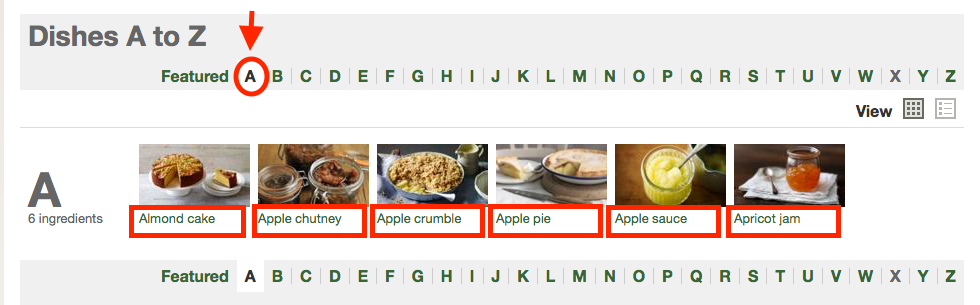
\includegraphics[width=10cm, height=5.5cm]{./report_file/4_1_1_ex.png}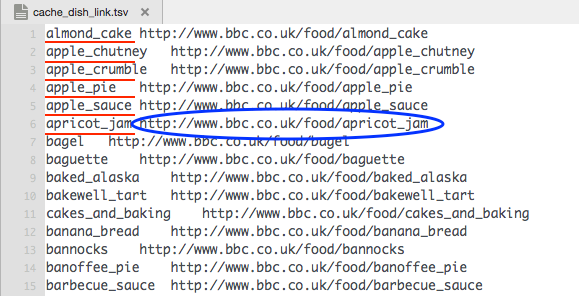
\includegraphics[width=10cm, height=5.5cm]{./report_file/cache_dish_link.png}
		\begin{flushright}\href{run:./report_file/cache_dish_link.tsv}{Open the entire file}\end{flushright}
		% 4.1.2
		\item	Once we have the link of a dish, we need to get all the recipes for this dish, but also all the recipes that use this dish. In order to do that, we crawl the pages found in the first step and we get the link where all the recipe links are listed. We store the web pages that contain the recipe links list likewise in the first step, with a pair <dish, link>.
		\\\\
		\hspace*{-0.5in}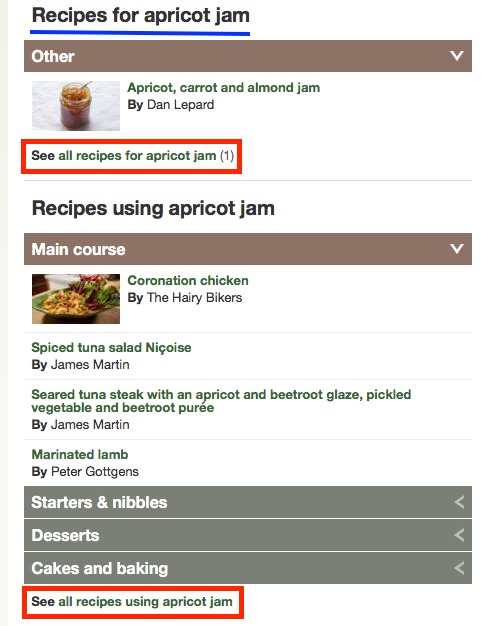
\includegraphics[width=8.5cm, height=7.5cm]{./report_file/4_1_2_ex.png}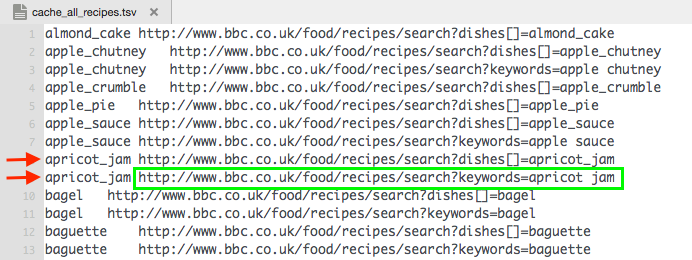
\includegraphics[width=8.5cm, height=6cm]{./report_file/cache_all_recipes.png}
		\begin{flushright}\href{run:./report_file/cache_all_recipes.tsv}{Open the entire file}\end{flushright}
		% 4.1.3
		\item The last part of this task consists in crawling the list of recipes for each link found in the previous phase. As can be seen in the figure below, every list has different size: the crawling must finish when the last page has been elaborated. The application acts in order to not save the same recipe link, that can be found under different dishes.
		\\\\
		\hspace*{-1.2in}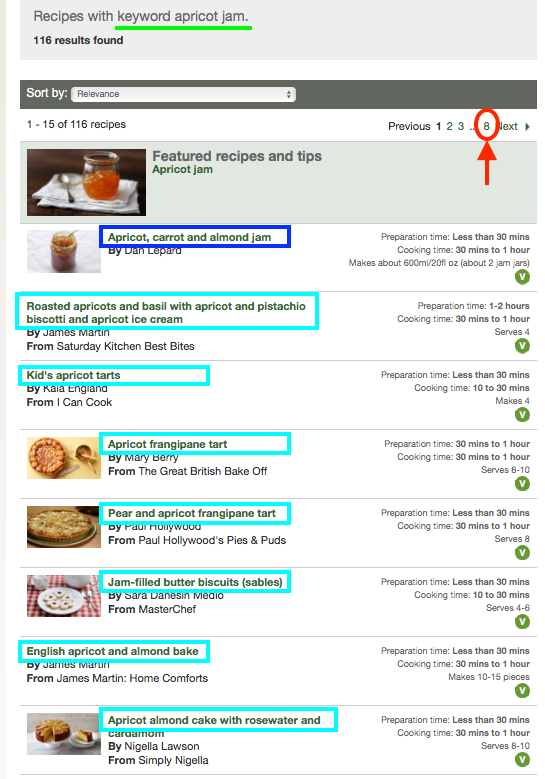
\includegraphics[width=8.5cm, height=10.5cm]{./report_file/4_1_3_ex.png}
		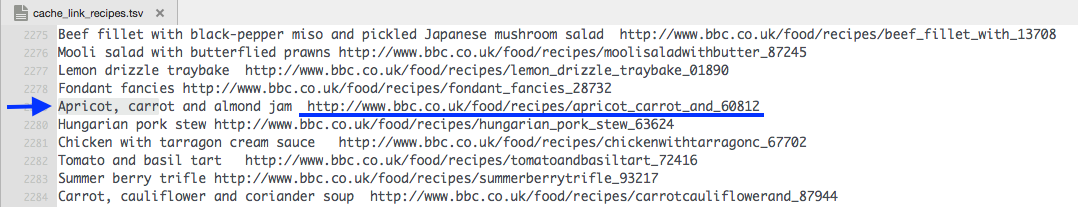
\includegraphics[width=15cm, height=5cm]{./report_file/cache_link_recipes.png}
		\begin{flushright}\href{run:./report_file/cache_link_recipes.tsv}{Open the entire file}\end{flushright}
	\end{enumerate}
	At the end of these three steps we have all the recipe available links on the web site, that must be elaborated in order to get the fondametal data for our recipe search engine.

	\subsection{Preprocess recipes}
	%TODO preprocess recipes
	\subsection{Build a search-engine index}
	%TODO build a search engine index


\end{document}
